\documentclass{simple}

\title[Despre calibrare]{Despre calibrare: O abordare structurată}
\institute{InfoEducație 2025 (CNU, Focșani)}
\author[Răzvan Deaconescu]{Răzvan Deaconescu \\
razvan.deaconescu@upb.ro}
\date{29 iulie 2025}

\begin{document}

\frame{\titlepage}

\begin{frame}{}
  \begin{figure}
    \centering
    
\includegraphics[width=0.7\textwidth]{img/flirting-attempts.png}
  \end{figure}
\end{frame}

\begin{frame}{Calibration}
  \begin{figure}
    \centering
    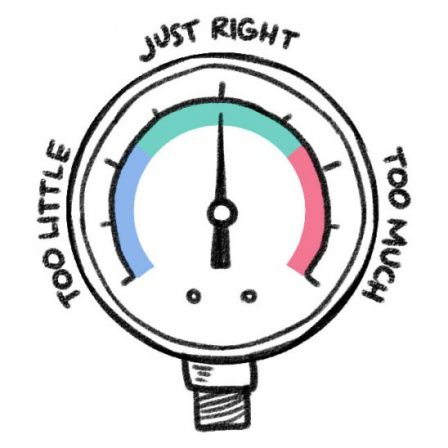
\includegraphics[width=0.7\textwidth]{img/calibration.jpg}
  \end{figure}
\end{frame}

\begin{frame}{Calibration (2)}
  \begin{figure}
    \centering
    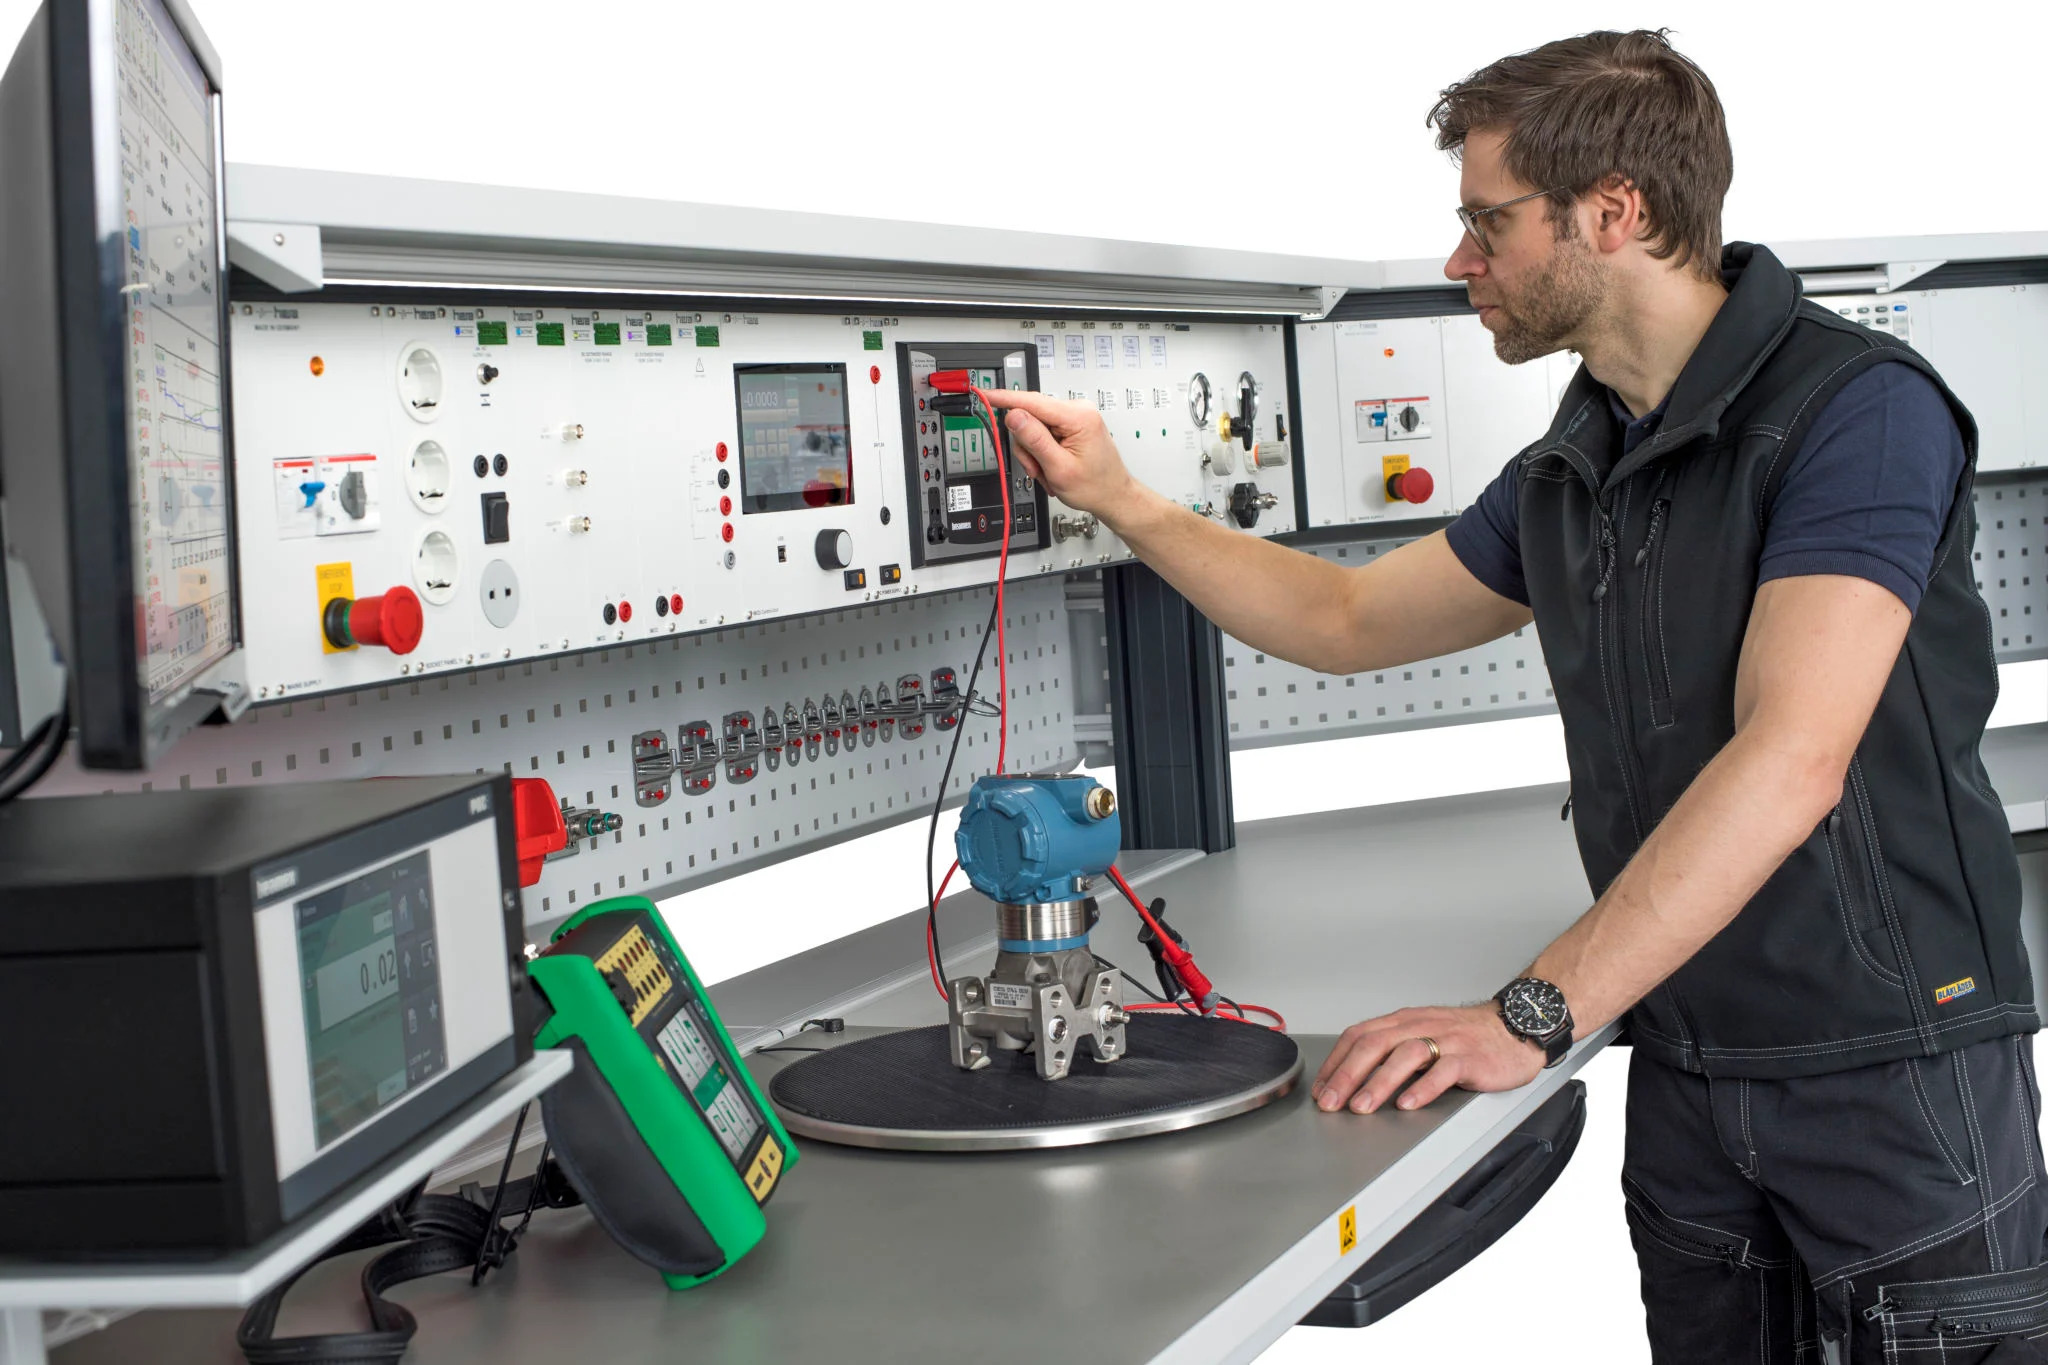
\includegraphics[width=0.9\textwidth]{img/calibration-engine.jpg}
  \end{figure}
\end{frame}

\begin{frame}{Calibrare socială}
  \centering
  \pause Cum interacționăm cu alții \\
  \vspace{3mm}
  \pause Cum ajungem să ne integrăm \\
  \vspace{3mm}
  \pause Cum ajungem să fim plăcuți \\
  \vspace{3mm}
  \pause Cum ajungem să obținem lucruri (favoruri, bani, apreciere, intimitate)
\end{frame}

\begin{frame}{}
  \begin{figure}
    \centering
    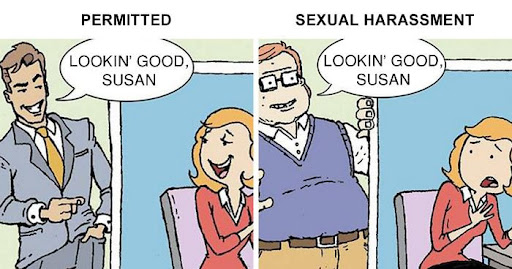
\includegraphics[width=0.9\textwidth]{img/looking-good-susan.jpg}
  \end{figure}
\end{frame}

\begin{frame}{}
  \begin{figure}
    \centering
    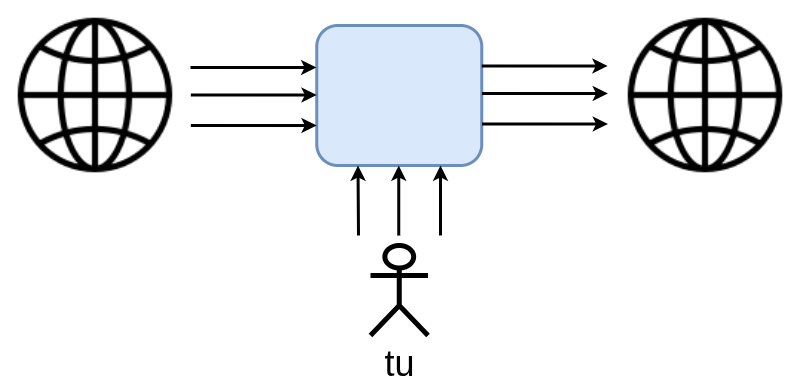
\includegraphics[width=0.9\textwidth]{img/calibration-input-output.png}
  \end{figure}
\end{frame}

\begin{frame}{}
  \begin{enumerate}
    \pause \item observe
    \pause \item calibrate
    \pause \item act
  \end{enumerate}
\end{frame}

\begin{frame}{Dar stai?}
  \centering
  \pause Nu e cam ingineresc? \\
  \vspace{3mm}
  \pause Lumea nu merge așa, mecanic, ca un model. \\
  \vspace{3mm}
  \pause Nu avem rețete, nu suntem roboți, trebuie să ,,simțim''.
\end{frame}

\begin{frame}{Da. Dar \ldots{}}
  \centering
  \pause Lumea e prea emoțională. \\
  \vspace{3mm}
  \pause Lumea e prea nestructurată. \\
  \vspace{3mm}
  \pause Lumea ar merita calibrată mai mult în partea de structură.
\end{frame}

\begin{frame}{}
  \begin{figure}
    \centering
    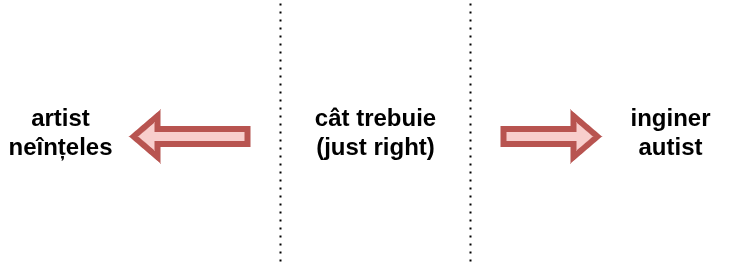
\includegraphics[width=0.8\textwidth]{img/inginer-artist.png}
  \end{figure}
\end{frame}

\begin{frame}{Cel mai bun răspuns}
  \centering
  \Large
  \pause depinde
\end{frame}

\begin{frame}{Calibrarea: Abordare matematică}
  \centering
  \Large
  \pause \texttt{f(x, y, z, \ldots{}) = r}
  \vspace{3mm}
  \pause Ce este \texttt{r}?
  \vspace{3mm}
  \pause Ce sunt \texttt{x, y, z, \ldots{}}?
  \vspace{3mm}
  \pause Ce este \texttt{f}?
\end{frame}

\begin{frame}{r - Rezultate}
  \begin{itemize}
    \pause \item apreciere
    \pause \item integrare socială
    \pause \item bani, resurse
    \pause \item intimitate
    \pause \item persuasiune
    \pause \item educație
    \pause \item manipulare
  \end{itemize}
\end{frame}

\begin{frame}{x, y, z, \ldots{} - ,,Butoanele''}
  \begin{itemize}
    \pause \item profilul, personalitatea ta
    \pause \item profilul, personalitatea celuilalt / celorlalți
    \pause \item poziția, reputația ta
    \pause \item poziția, reputația celuilalt / celorlalți
    \pause \item starea ta
    \pause \item starea celuilalt / celorlalți
    \pause \item circumstanțele: locul, timpul, starea lumii, zeitgeist-ul
  \end{itemize}
\end{frame}

\begin{frame}{Control}
  \begin{figure}
    \centering
    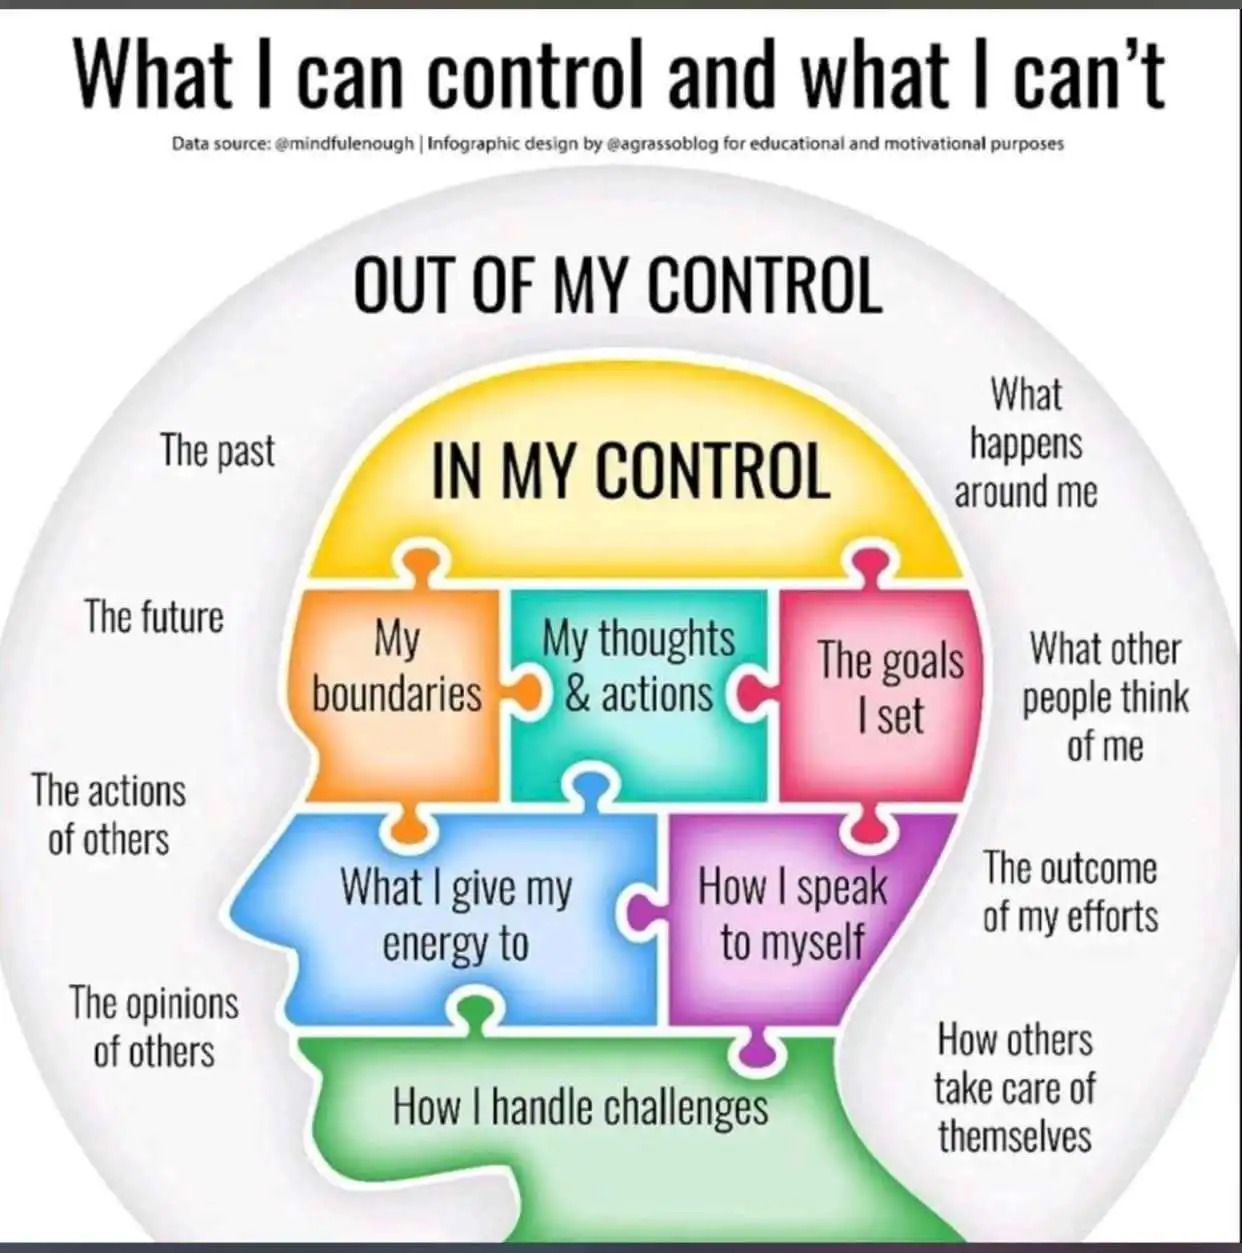
\includegraphics[width=0.7\textwidth]{img/control.jpg}
  \end{figure}
\end{frame}

\begin{frame}{Chiar dacă nu controlezi poți să \ldots{}}
  \centering
  \pause observi \\
  \vspace{3mm}
  \pause analizezi \\
  \vspace{3mm}
  \pause stabilești relații de tip cauză-efect \\
  \vspace{3mm}
  \pause influențezi
\end{frame}

\begin{frame}{Inner vs. Outer Game}
  \begin{figure}
    \centering
    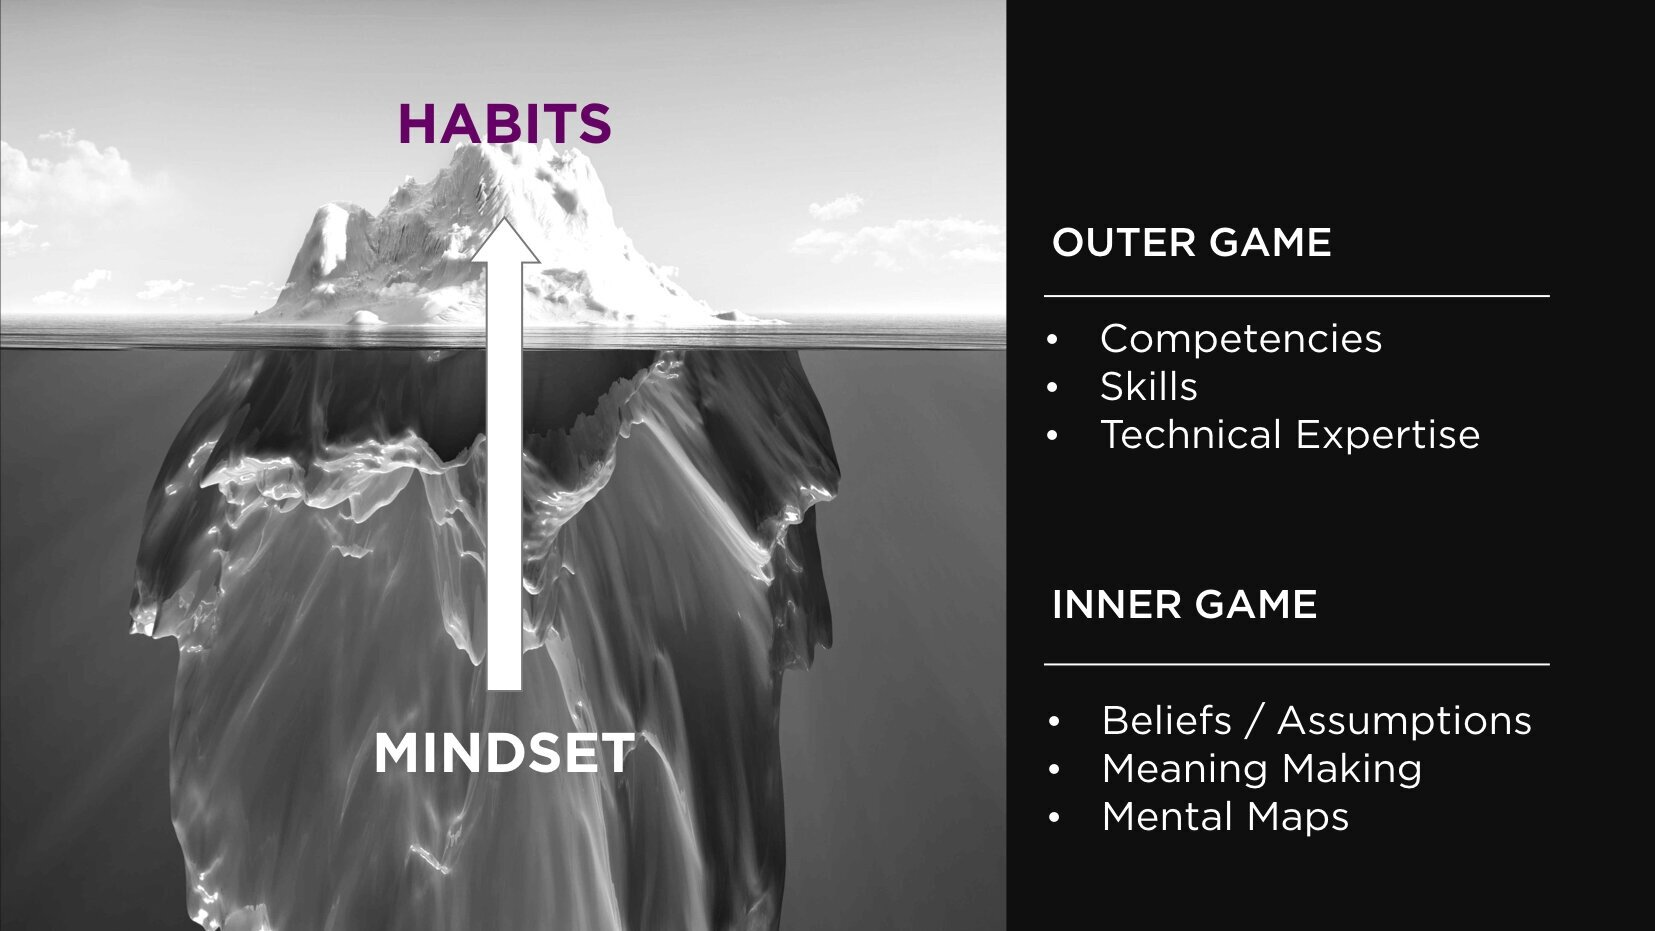
\includegraphics[width=0.9\textwidth]{img/inner-outer-game}
  \end{figure}
\end{frame}

\begin{frame}{f - Calibrarea, acțiunea, abordarea}
  \begin{itemize}
    \pause \item no silver bullet
    \pause \item iterație + feedback + îmbunătățire
  \end{itemize}
\end{frame}

\begin{frame}{Ce au în plus oamenii mai în vârstă?}
  \begin{itemize}
    \pause \item experiență (socială)
    \pause \item capital social-politic, conexiuni
  \end{itemize}
\end{frame}

\begin{frame}{Cum ajungi ,,calibrat''?}
  \begin{itemize}
    \pause \item numai cine nu muncește, nu greșește
    \pause \item încerci, greșești, re-încerci
    \pause \item o să o dai în bară, o să greșești, o să fii respins
    \pause \item \textit{If you don't cringe about your past, did you really evolve?}
  \end{itemize}
\end{frame}

\begin{frame}{Mindset de ,,calibrare''}
  \begin{itemize}
    \pause \item Nimeni nu s-a născut expert.
    \pause \item Partea socială nu e ceva care e ,,de neatins''. Nu e ,,locul 1 la 100m''.
    \pause \item Se educă.
  \end{itemize}
\end{frame}

\begin{frame}{Diferențe între \ldots{}}
  \begin{itemize}
    \pause \item profesor
    \pause \item coach / antrenor
    \pause \item mentor
  \end{itemize}
\end{frame}

\begin{frame}{Framework de educație și calibrare}
  \begin{itemize}
    \pause \item Observi.
    \pause \item Încerci în mediu controlat.
    \pause \item Încerci în lumea largă - în pași mici.
    \pause \item Try. Fail. Try again. Fail better.
    \pause \item Dezvolți rezistență la eșec, respingere. Dar nu ignori, înveți, iei feedback.
    \pause \item Try. Rinse. Repeat.
  \end{itemize}
\end{frame}

\begin{frame}{}
  \begin{enumerate}
    \pause \item observe
    \pause \item calibrate
    \pause \item act
    \pause \item goto step 1
  \end{enumerate}
\end{frame}

\begin{frame}{Ce e de făcut?}
  \begin{itemize}
    \pause \item încercați
    \pause \item încercați lucruri noi
    \pause \item încercați lucruri noi în doze mici de noutate
    \pause \item faceți cât mai multe lucruri cu alți oameni
    \pause \item o veți da în bară, obișnuiți-vă cu ideea
    \pause \item Try. Rinse. Repeat.
    \pause \item căutați-vă mentori
  \end{itemize}
\end{frame}

\begin{frame}{Referințe}
  \begin{itemize}
    \pause \item Robert Cialdini: \textit{Influence: The Psychology of Persuasion}
    \pause \item Allan Pease: \textit{The Definitive Book of Body Language: The Secret Meaning Behind People's Gestures}
    \pause \item Try. Fail. Repeat. Fail better.
    \pause \item Try. Rinse. Repeat.
    \pause \item \url{https://www.slideshare.net/razvandeaconescu}
    \pause \item \url{https://github.com/razvand/slides/tree/master/despre-calibrare}
  \end{itemize}
\end{frame}

\end{document}
